\documentclass[letterpaper,12pt]{article}
\usepackage{tabularx} % extra features for tabular environment
\usepackage{amsmath}  % improve math presentation
\usepackage{float}
\usepackage{pdfpages}

\usepackage{graphicx} % takes care of graphic including machinery
\graphicspath{ {./figures/} }
\usepackage[margin=1in,letterpaper]{geometry} % decreases margins
\usepackage{cite} % takes care of citations
\usepackage[final]{hyperref} % adds hyper links inside the generated pdf file
\hypersetup{
	colorlinks=true,       % false: boxed links; true: colored links
	linkcolor=blue,        % color of internal links
	citecolor=blue,        % color of links to bibliography
	filecolor=magenta,     % color of file links
	urlcolor =blue         
}

%



\begin{document}

\title{Experiment 7 Preliminary Work \protect\\ Rectifiers, Capacitors  and Inductors}
\author{Ahmet Akman 2442366 \protect\\}
\date{\today}
\maketitle
\newpage
\tableofcontents
\newpage
%\begin{abstract}
%abstract
%\end{abstract}

\section*{Introduction} 
In preliminary work of the Experiment 7 , the steps for the pre-experiment are conducted and presented.
\section{1.}
Introduction to Basic Circuit Elements and Notes on Diodes documents are studied and necessary points are noted.
\section{2.}

For this step circuits given in Figure 1 and 2 are taken as the reference and built in simulation environment
\begin{figure}[H]
	\centering
   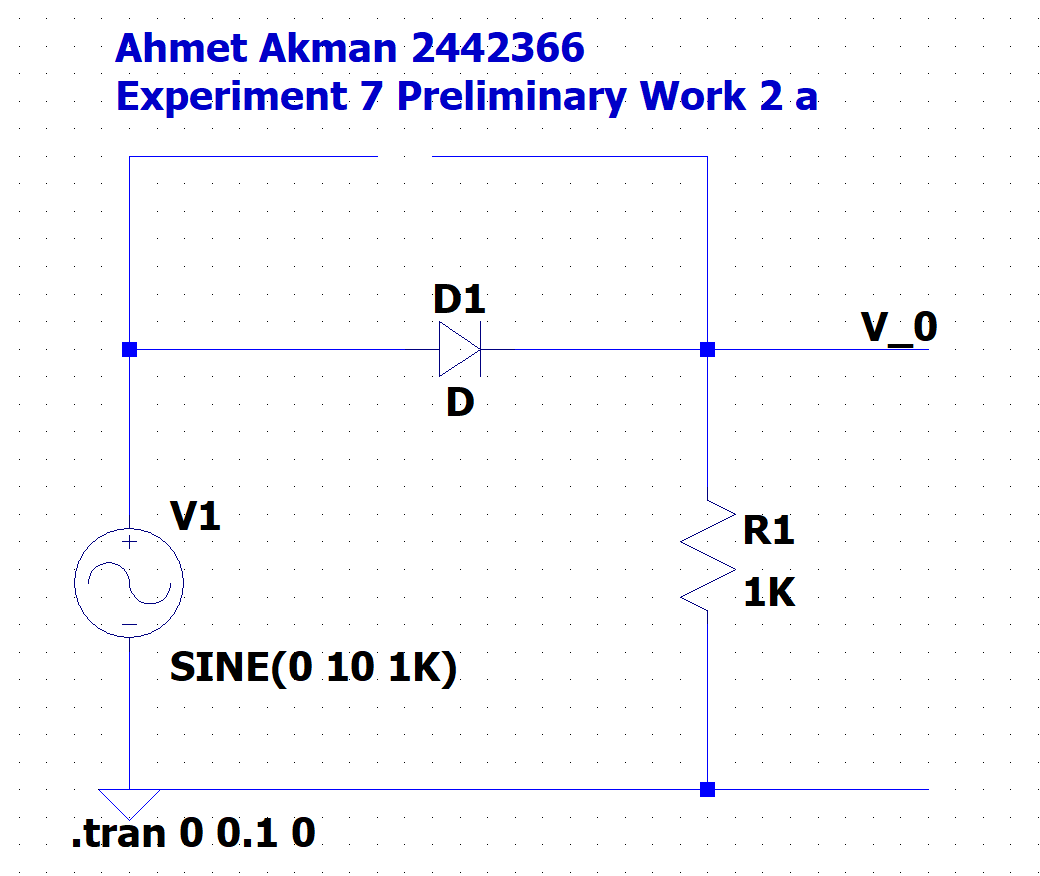
\includegraphics[width=1\textwidth]{Pre1a_sch.png}
   \caption{Simulation schematic for the step 1 half-wave rectifier}
\end{figure} 
\begin{figure}[H]
	\centering
   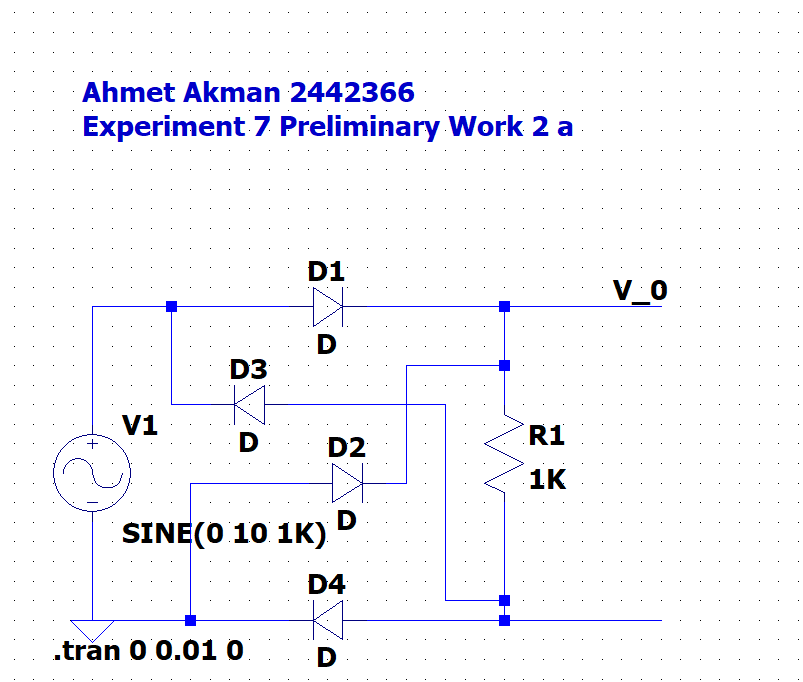
\includegraphics[width=1\textwidth]{Pre1a2_sch.png}
   \caption{Simulation schematic for the step 1 full-wave rectifier}
\end{figure} 

\subsection{a)}
In this subsection circuits in the Figure 1 and Figure 2 are simulated for the same input voltage as \(V_{in} \) = \(10sin(2000\pi t)\)V and load resistance as 1k\(\Omega\). The output voltages are \(V_0\)(t). The results are given in Figures 3 and 4.
\begin{figure}[H]
	\centering
   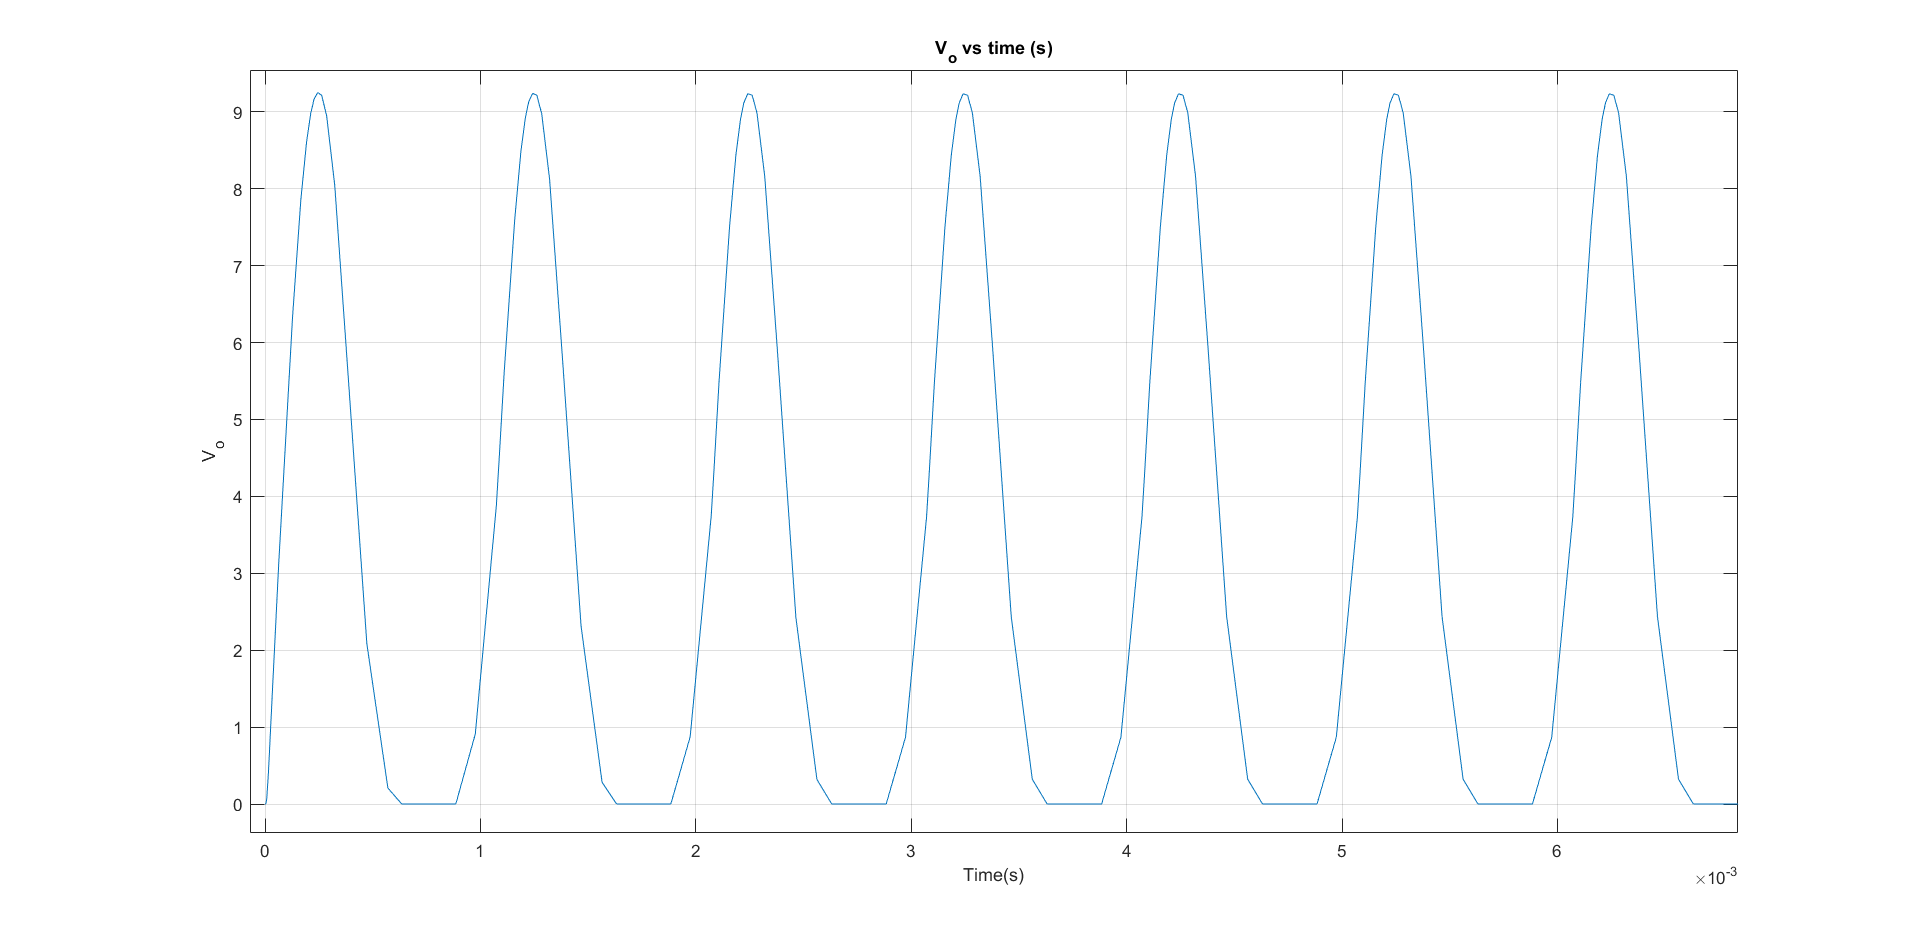
\includegraphics[width=1\textwidth]{PRE_2a.png}
   \caption{Simulation result for the circuit in Figure 1}
\end{figure} 
\begin{figure}[H]
	\centering
   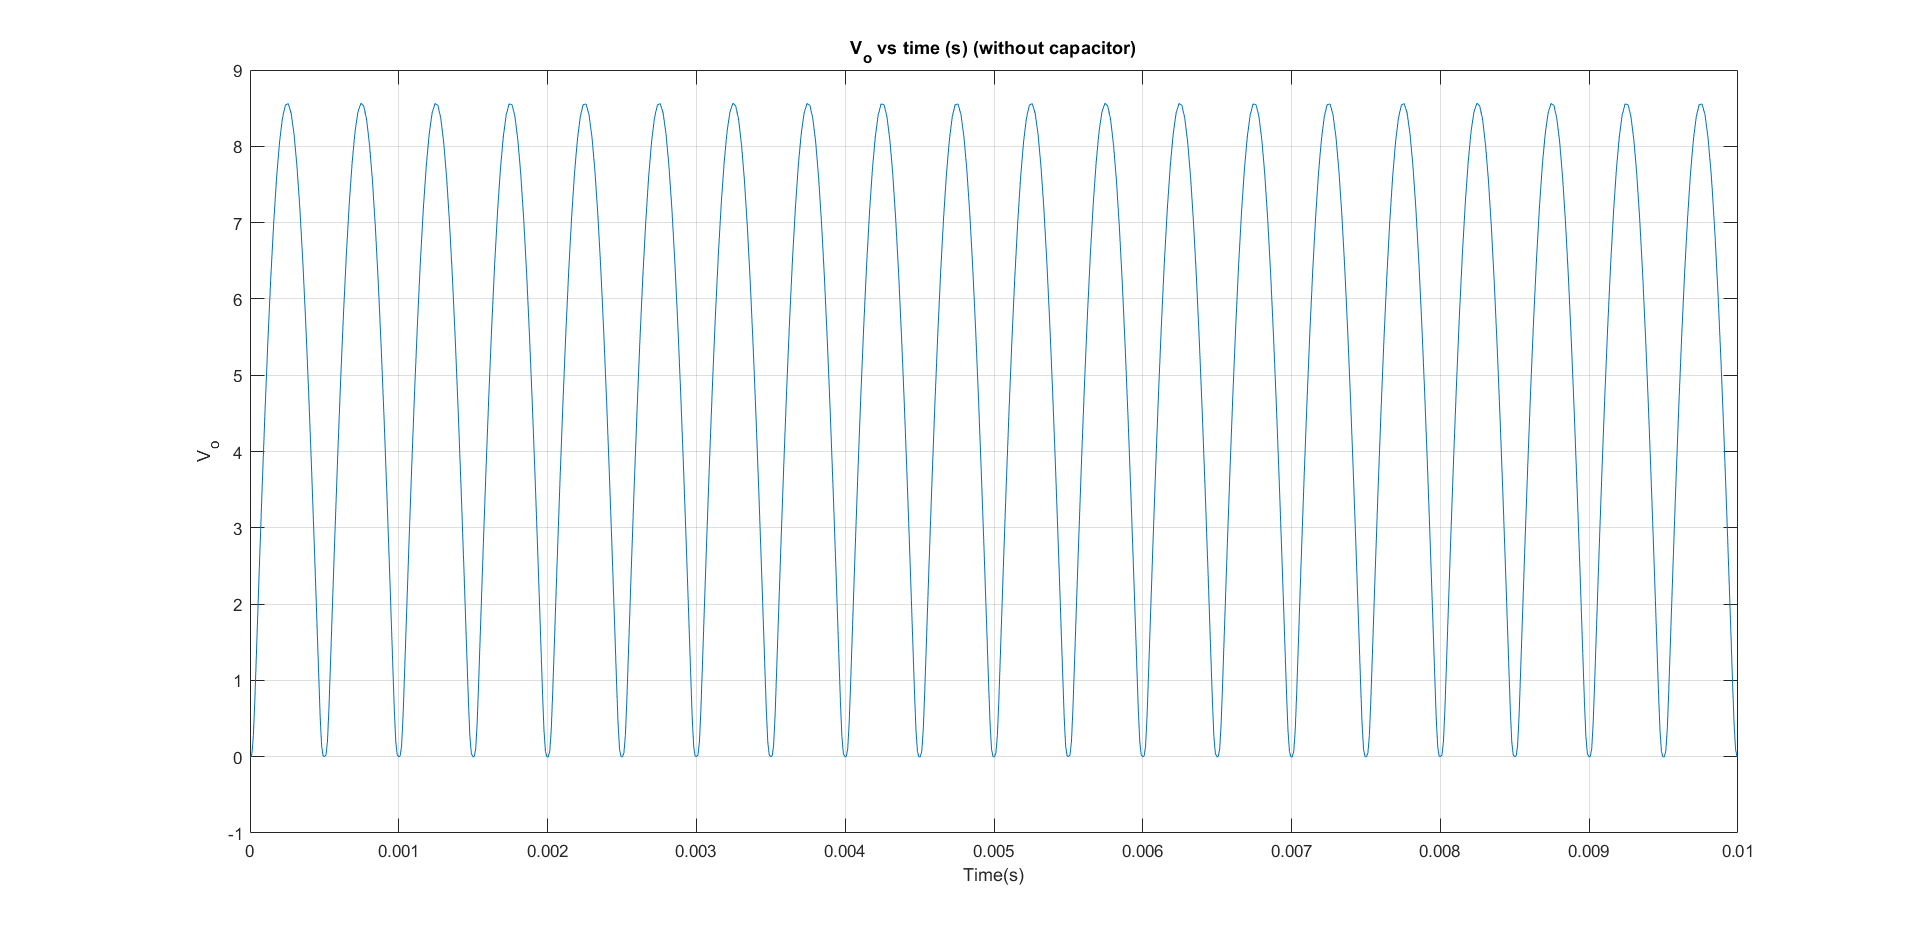
\includegraphics[width=1\textwidth]{2a2_plot.png}
   \caption{Simulation result for the circuit in Figure 2} 
\end{figure} 
It can be stated that half wave rectifier only allows the current flow when it is positive and creates flat regions when it is negative. On the other hand, full wave rectifier allows current flow continously in positive region by the virtue of diodes without creating flat regions.
\subsection{b)}
The circuit schematic given in Figure 5 is constructed in LTSPice environment .
\begin{figure}[H]
	\centering
   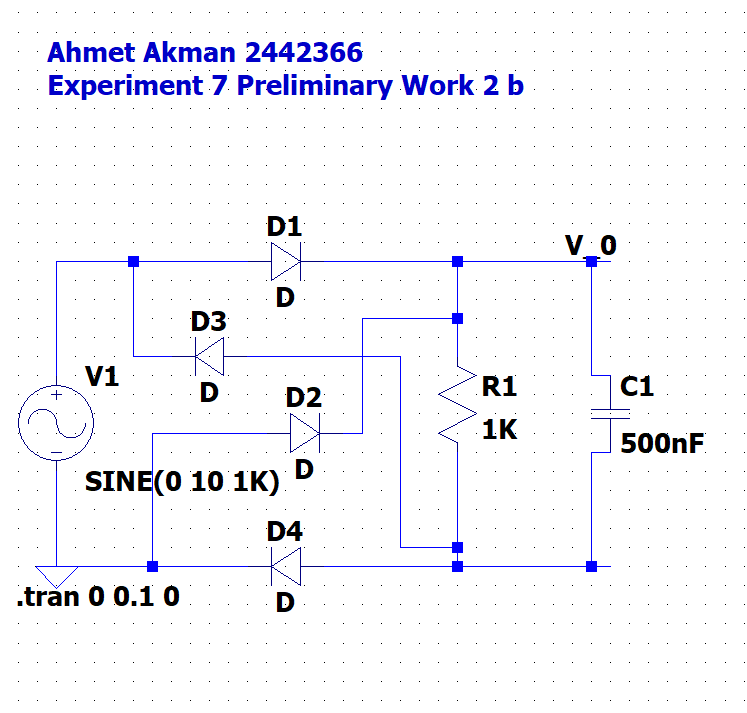
\includegraphics[width=1\textwidth]{Pre1b_sch.png}
   \caption{Simulation schematic for the part b}
\end{figure} 

Simulation is repeated with capacitance values of 1\(\mu F\) and 500nF.
The output of the circuit  with 1\(\mu F\) capacitor is shown in Figure   6.
\begin{figure}[H]
	\centering
   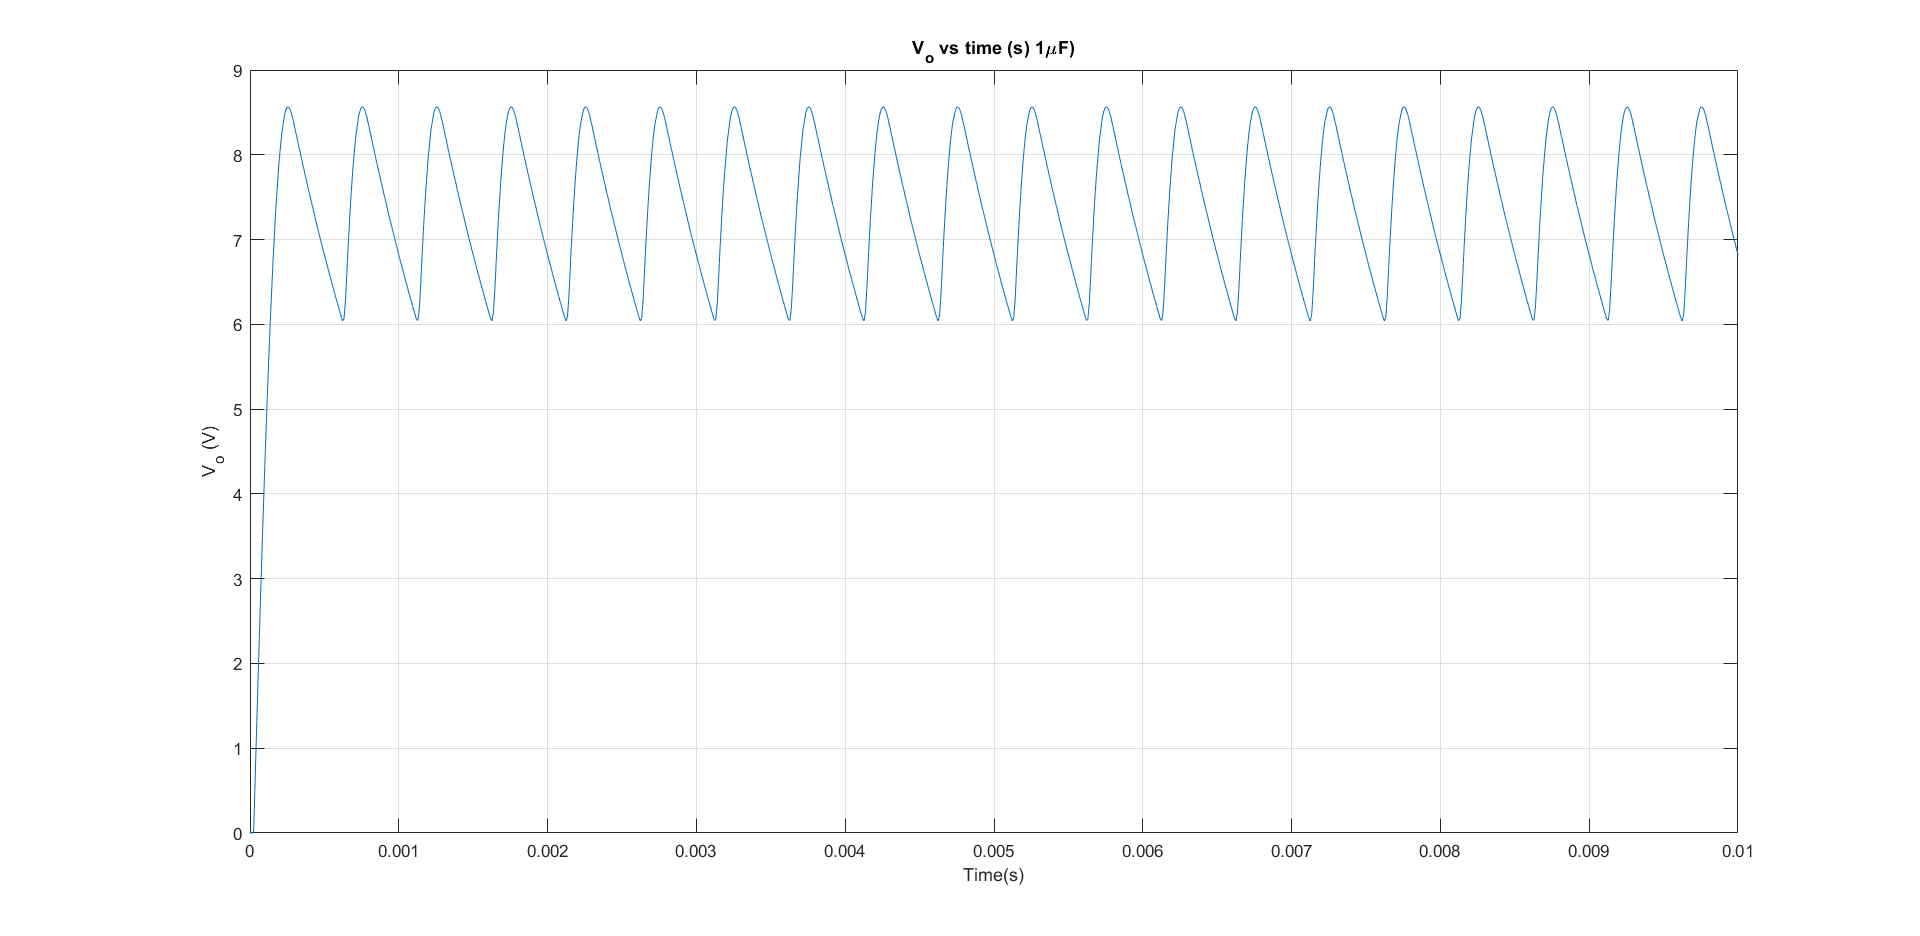
\includegraphics[width=1\textwidth]{PRE_2b_1uF.png}
   \caption{First simulation result for the circuit in Figure 5}
\end{figure} 

The output of the circuit  with 500nF capacitor is shown in Figure   7.
\begin{figure}[H]
	\centering
   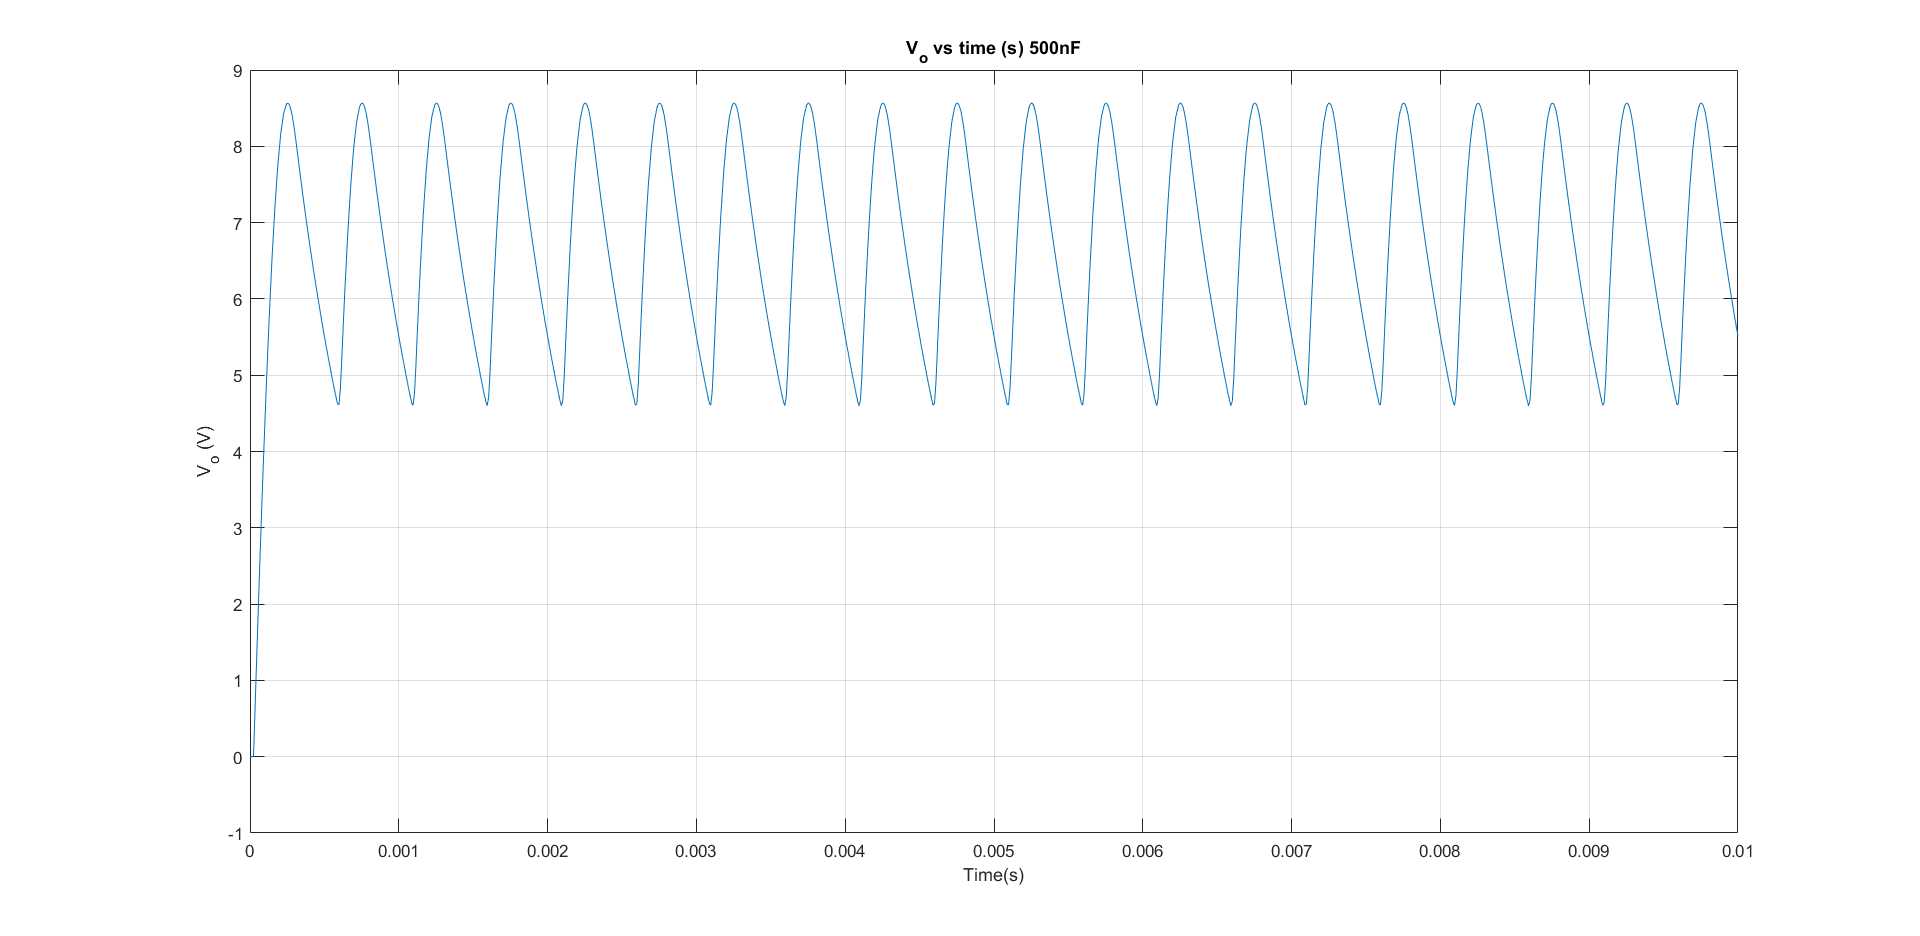
\includegraphics[width=1\textwidth]{PRE_2b_500nF.png}
   \caption{Second simulation result for the circuit in Figure 5}
\end{figure} 
It is observed that higher capacitance would make ripple voltage lower and helps rectifier to have more like DC output.
\section{3.}
The circuit given in Figure 8 is considered to obtain the capacitance of the capacitor expresssion.
\begin{figure}[H]
	\centering
   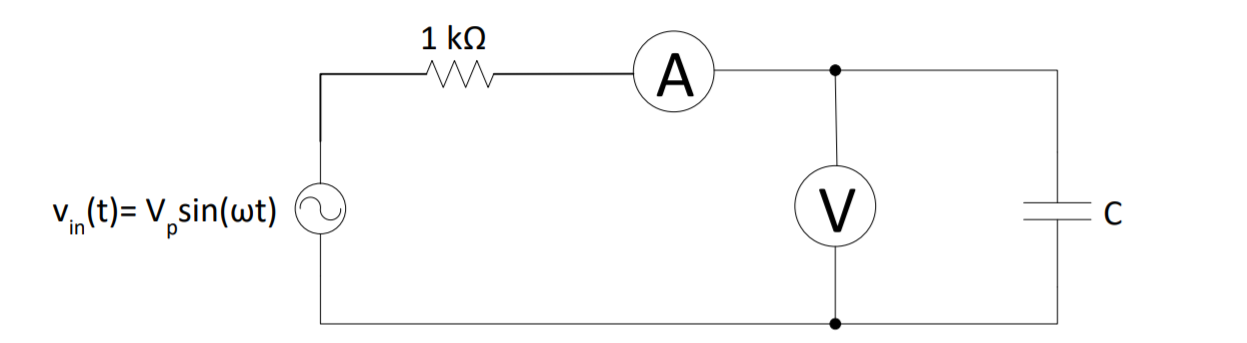
\includegraphics[width=1\textwidth]{PRE3.png}
   \caption{Circuit schematic for Step 3}
\end{figure} 
The expression is obtained as follows,
\[|z_c| = \frac{1}{\omega C} = \frac{V_{RMS}}{i_{RMS}}\]
so,
\[C = \frac{i_{RMS}}{V_{RMS} \omega}
	\]


\section{4.}
For this section circuit schematic given in Figure 9 is taken as the reference.
\begin{figure}[H]
	\centering
   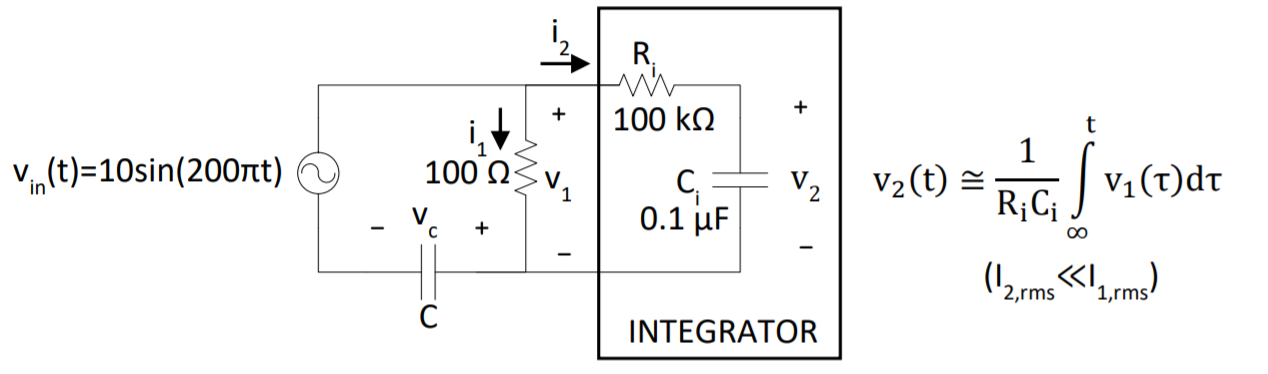
\includegraphics[width=1\textwidth]{PRE4.png}
   \caption{Circuit schematic for Step 4}
\end{figure} 
\subsection{a)}
The equation relating charge q and the capacitance of the capacitor C in terms of \(V_2\) and \(V_c\) is obtained as follows,
\[ i_2(t) = C_1 \frac{d V_2}{dt} = \frac{V_1(t)}{R_1}
\]
\[
	V_2(t) = \frac{1}{R_i C_i} * \int_{-\inf}^{t} V_1(\tau) \, d\tau
	\]
	\[
		V_2(t) = \frac{R}{R_i C_i} * \int_{-\inf}^{t} i_1(\tau) \, d\tau
		\]
So, 
\[ q(t) = C V_c(t) = \int_{-\inf}^{t} i_1(\tau) \,\tau = \frac{R_i C_i V_2(t)}{R} \]
\subsection{b)}
The q-v characteristics can be obtained by connecting one probe of the DSO to the \(V_2\) and another one to the \(V_c\). Then using math operations and XY display mode q-v can be obtained on the screen of the DSO.
\subsection{c)}
The verification the technique given in the subsection b) can be illustrated using the simulation circuit as shown in Figure 10.
\begin{figure}[H]
	\centering
   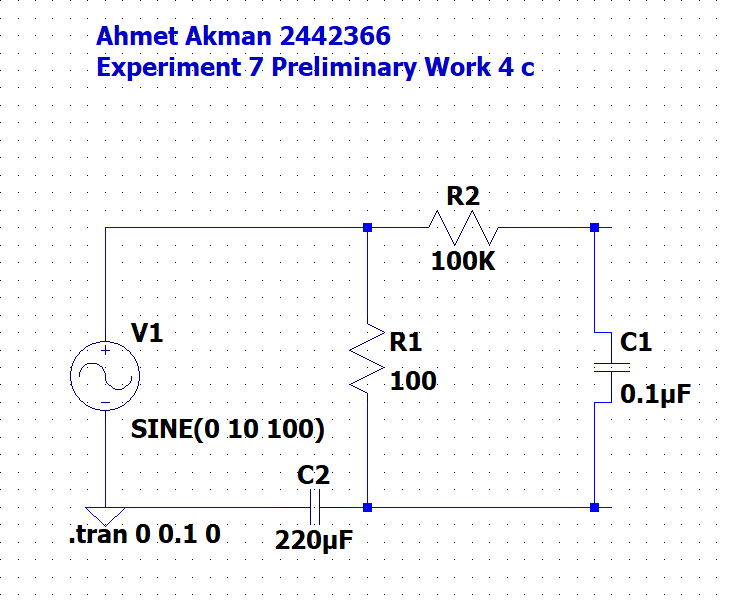
\includegraphics[width=1\textwidth]{Pre4c_sch.png}
   \caption{Circuit schematic for capacitance finding method}
\end{figure} 
Capacitor value is used as 220 \(\mu\)F and the result is obtained in MATLAB (data is fetched from the LTSPice) given in Figure 11.
\begin{figure}[H]
	\centering
   \includegraphics[width=1\textwidth]{PRE_4C.png}
   \caption{The q-v characteristics plot}
\end{figure} 
\section{5.}
The resistance of the actual inductor can be measured via measuring both \(i_{RMS}\) and \(V_{RMS}\) values then dividing  \(V_{RMS}\) to \(i_{RMS}\).
\[ R = \frac{V_{RMS}}{i_{RMS} } \]
\section{6.}
The inductance value L can be expressed in terms of measured rms current and voltages , the angular frequency \(\omega\) , and the resistance r as follows,
\[|Z_c| = \omega L = \frac{V_{RMS}}{i_{RMS}}\]
so,
\[C = \frac{V_{RMS} \omega}{i_{RMS}}
	\]
\section{7.}
	For this section circuit schematic given in Figure 12 is taken as the reference.
	\begin{figure}[H]
		\centering
	   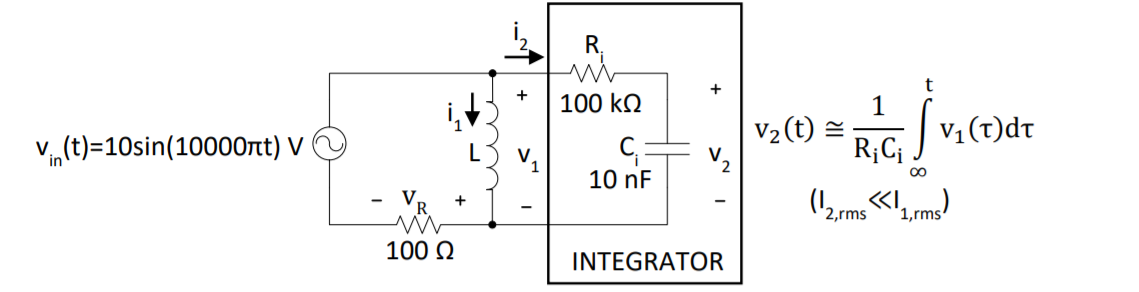
\includegraphics[width=1\textwidth]{PRE7.png}
	   \caption{Circuit schematic for Step 7}
	\end{figure} 
	\subsection{a)}
	The equation relating flux \(\phi\) and the inductance of the inductor L in terms of \(V_2\) and \(V_r\) is obtained as follows,
\[
i_1*100 = V_R
\]
\[
	\phi(t) = L i(t) = \frac{L V_R}{100}
\]
by the equation given in Figure 12,
\[V_2 R_i C_i = L i(t)\]
\[V_2 R_i C_i = \frac{L V_R}{100}\]
\[L = \frac{100 V_2 R_i C_i}{V_R}\]
also,
\[\phi(t) = V_2 R_i C_i\]
\subsection{b)}

The \(\phi-i\) characteristics can be obtained on DSO using the setup given in Figure 12 via applying following steps. First the channels of the DSO should be connected to measure \(V_2\) and \(V_R\). Then using the mathematical expressions given in section a, and the math opeartions of the DSO the \(\phi-i\) characteristics can be obtained on DSO screen.
\subsection{c)}
The verification the technique given in the subsection b) can be illustrated using the simulation circuit as shown in Figure 13.
\begin{figure}[H]
	\centering
   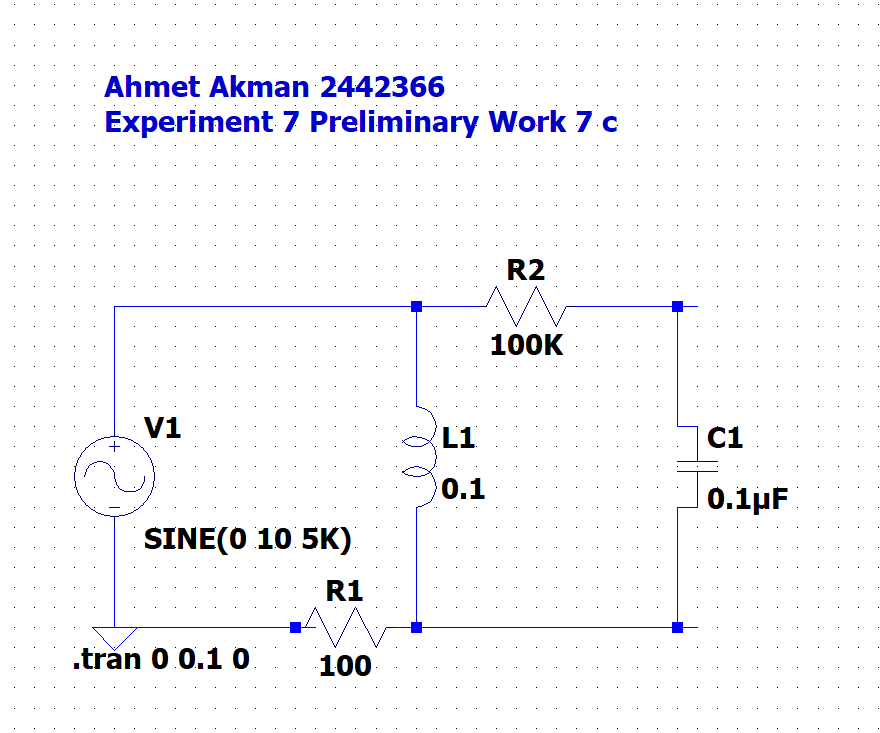
\includegraphics[width=1\textwidth]{Pre7c_sch.png}
   \caption{Circuit schematic for inductance finding method}
\end{figure} 
Inductance value is used as 0.1 \(\mu\)H and the result is obtained in MATLAB (data is fetched from the LTSPice) given in Figure 14.
\begin{figure}[H]
	\centering
   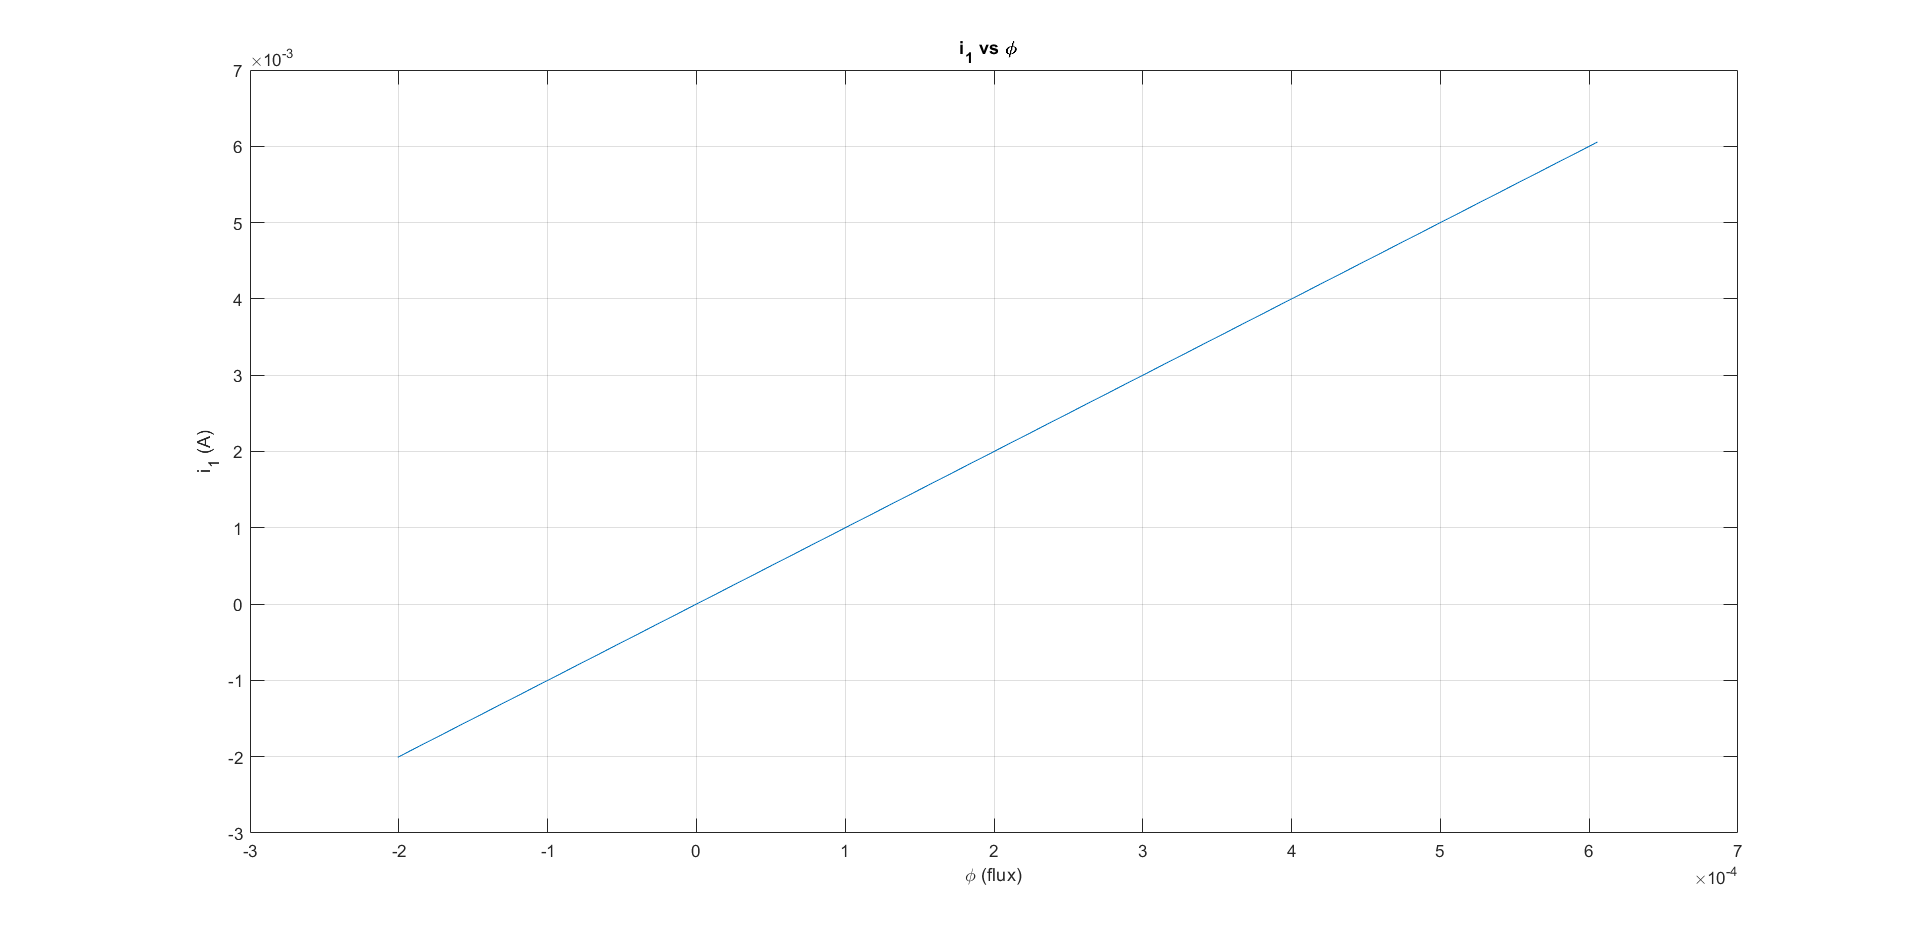
\includegraphics[width=1\textwidth]{PRE_7c.png}
   \caption{The \(\phi\)-i characteristics plot}
\end{figure} 

\section*{Conclusion}
In conclusion, in preliminary work of experiment 7, "Rectifiers, Capacitors and Inductors"  needed the expressions for the integrator circuits are obtained and necessary data are plotted using those relations. Then and simulations are made and compared with theoretical results.

%++++++++++++++++++++++++++++++++++++++++
% References section will be created automatically 
% with inclusion of "thebibliography" environment
% as it shown below. See text starting with line
% \begin{thebibliography}{99}
% Note: with this approach it is YOUR responsibility to put them in order
% of appearance.

%\begin{thebibliography}{99}

%https://tr.overleaf.com/latex/templates/sample-lab-report-for-u-of-r-phys-349/pgsyqngcyjxk

%\end{thebibliography}


\end{document}


\begin{table}[H]
	\begin{center}
		\caption{Resistance reading by color code convention.}
		\vspace{2mm}
		\begin{tabular}{||c | c | c||} 
		 \hline
		 Color Order & Value & Tolerance \\ [0.5ex] 
		 \hline\hline
		 Brown / Black / Red / Gold & 1k\( \Omega \) & \( \% \) 5  \\ 
		 \hline
		 Yellow / Violet / Red / Gold & 4.7k\( \Omega \) & \( \% \) 5   \\
		 \hline
		 Brown / Grey / Orange / Gold & 18k\( \Omega \) & \( \% \) 5  \\ [1ex] 
		 \hline
		\end{tabular}
	\end{center}
	\end{table}

	\begin{figure}[H]
 		\centering
		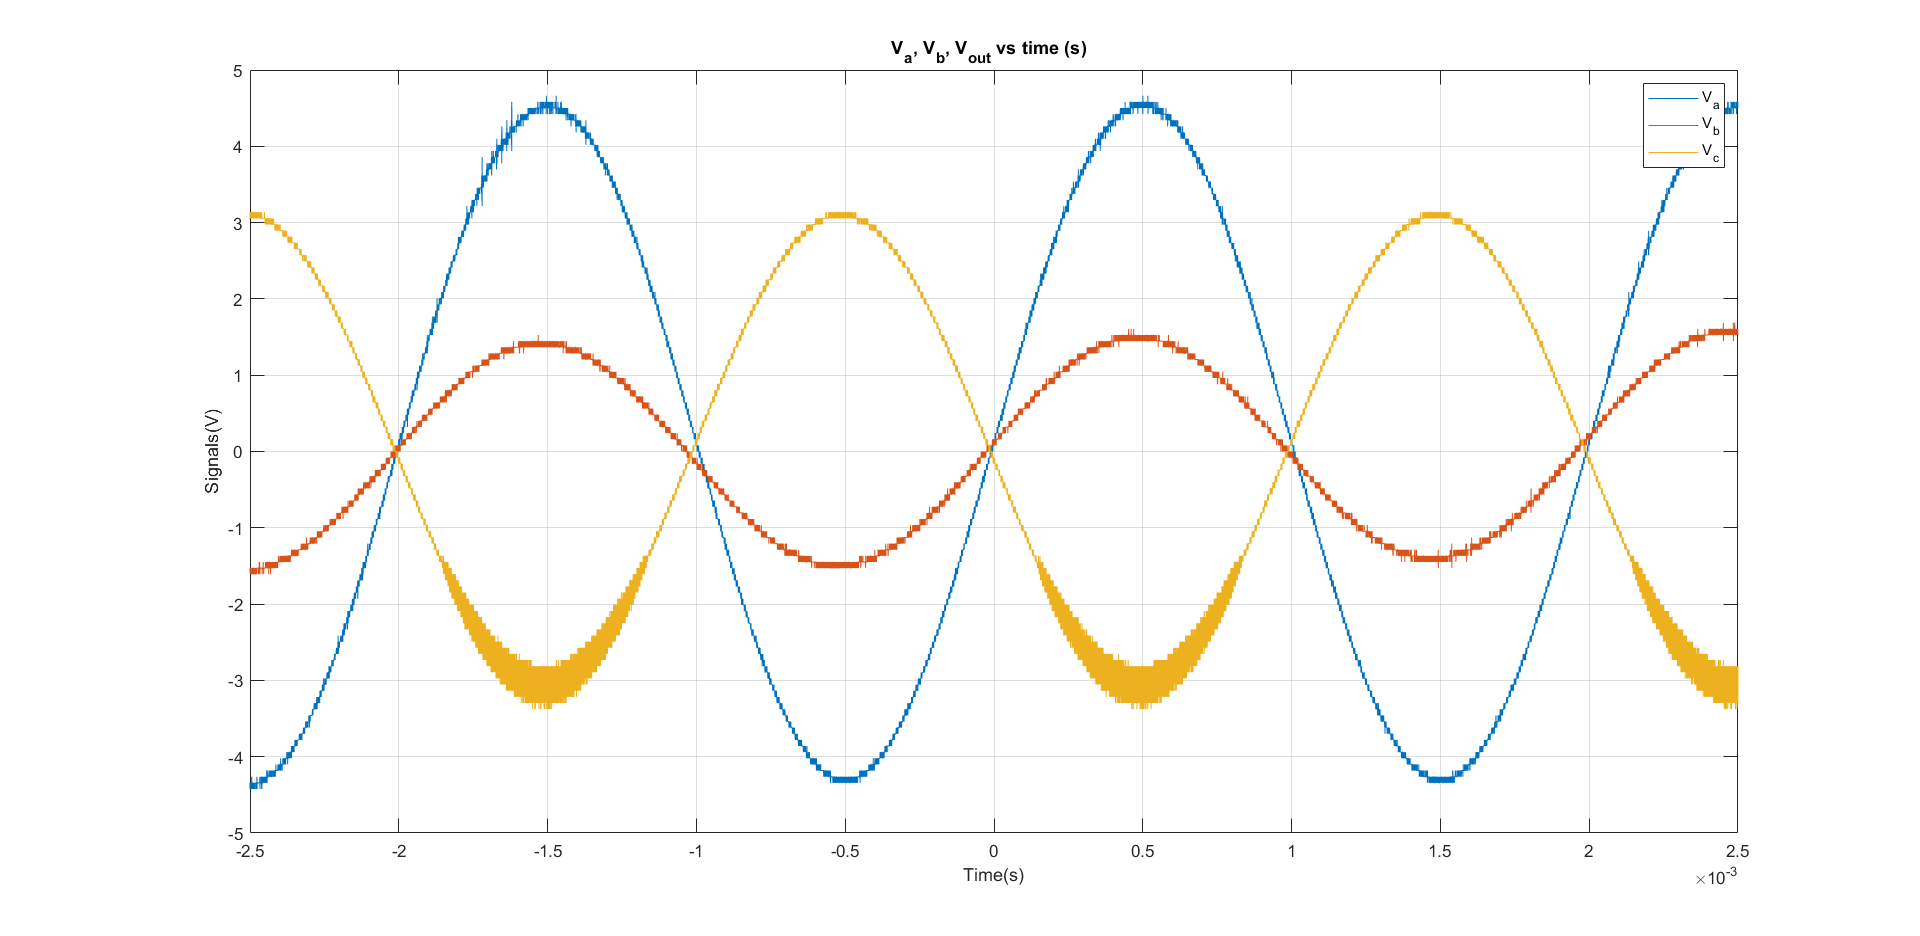
\includegraphics[width=0.6\textwidth]{5.png}
		\caption{Circuit schematic for the step 5}
	\end{figure} 

	\begin{figure}[htp] \centering{
		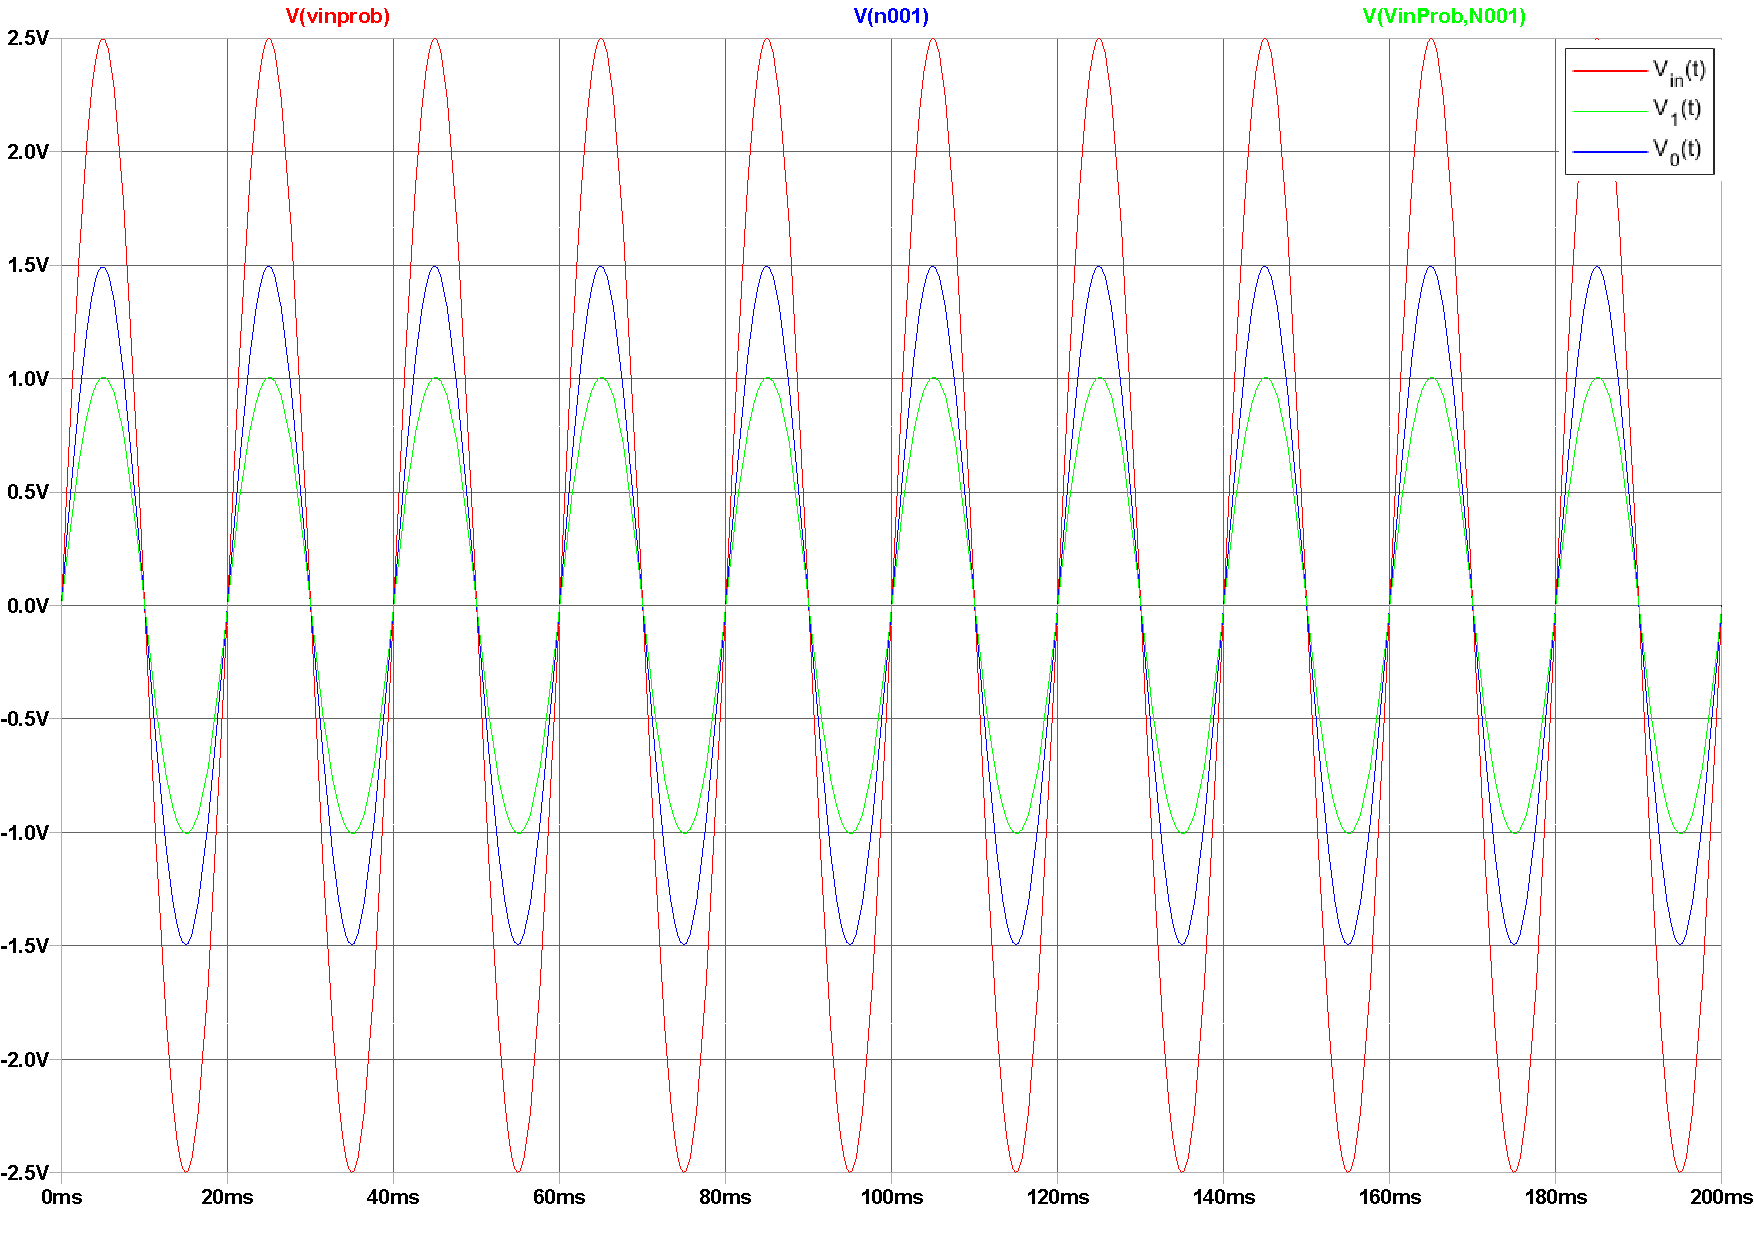
\includegraphics[scale=0.25]{2a_plot.pdf}}
		\caption{Experiment 2}
\end{figure}
	